\documentclass{article}
\title{A genetic classification of the tholeiitic\\
  and calc-alkaline magma series}
\author{Pieter Vermeesch\footnotemark[1]~ and Victoria Pease\footnotemark[2]\\
  \footnotemark[1] University College London\\
  \footnotemark[2] Stockholm University
}
\usepackage{graphicx,natbib,amsmath,lineno,fullpage}
\usepackage[hidelinks]{hyperref}
\begin{document}
\linenumbers
\maketitle

\begin{abstract}
  The concept of the `magma series' and the distinction between
  alkaline, calc-alkaline and tholeiitic trends has been a cornerstone
  in igneous petrology since the early 20\textsuperscript{th} century,
  and encodes fundamental information about the redox state of
  divergent and convergent plate tectonic settings. We show that the
  `Bowen and Fenner trends' that characterise the calc-alkaline and
  tholeiitic types of magmatic environments can be approximated by a
  simple logratio model based on three coupled exponential decay
  functions, for A = Na\textsubscript{2}O + K\textsubscript{2}O, F =
  FeO\textsubscript{T} and M = MgO, respectively.  We use this simple
  natural law to define a `Bowen-Fenner index' to quantify the degree
  to which an igneous rock belongs to either magma series.  Applying
  our model to a data compilation of igneous rocks from Iceland and
  the Cascade Mountains effectively separates these into tholeiitic
  and calc-alkaline trends.  However the simple model fails to capture
  the distinct dogleg that characterises the tholeiitic logratio
  evolution, which can be attributed to the switch from ferrous to
  ferric iron bearing minerals.  Parameterising this switch in a two
  stage magma evolution model results in a more accurate fit to the
  Icelandic data. The same two-stage model can also be fitted in
  A--T--M space, where `T' stands for TiO\textsubscript{2}. This
  produces a new way to identify calc-alkaline and tholeiitic rocks
  that does not require the conversion of FeO and
  Fe\textsubscript{2}O\textsubscript{3} to FeO\textsubscript{T}. Our
  results demonstrate that logratio analysis provides a natural way to
  parameterise physical processes that give rise to these magma
  series.
\end{abstract}

\section{Introduction}

Much petrological nomenclature predates plate tectonic theory.
Without an overarching theoretical paradigm to understand
petrogenesis, early 20\textsuperscript{th} century geologists relied
on empirical trends to classify rocks. But despite this lack of
theoretical understanding, several of these empirical models survived
the plate tectonic revolution and neatly fitted into a plate tectonic
context.\medskip

A case in point is the division of subalkaline igneous rocks into
tholeiitic and calc-alkaline suites. This classification has its roots
in the 1920s \citep{bowen1928, fenner1929, kennedy1933, tilley1950}
and is based on the empirical observation that, when plotting igneous
rocks on an A--F--M diagram (where A =
Na\textsubscript{2}O+K\textsubscript{2}O, F = FeO\textsubscript{T}, M
= MgO, and A + F + M = 1), magmatic differentiation can produce a
`Fenner trend' (F/M ratio increases with increasing A) or a `Bowen
trend' (the F/M ratio remains more constant). The Fenner and Bowen
trends characterise the tholeiitic and calc-alkaline suites,
respectively.\medskip

The difference between tholeiitic and calc-alkaline magma sources is
quite evidently related to their oxygen fugacity \citep{osborn1959}.
In reduced magmas, Fe is removed slowly by crystallisation of Mg-rich
ferrous minerals such as olivine and pyroxene. This results in an
increase of the Fe/Mg-ratio during the initial stages of magma
evolution, the tholeiitic suite of rocks. Oxidising conditions in a
parent magma promote the crystallisation of ferric-iron bearing
magnetite, which removes Fe more efficiently, producing the
calc-alkaline trend.\medskip

The division of igneous rocks into tholeiitic and calc-alkaline suites
makes sense in a plate tectonic context. Tholeiitic rocks are found at
mid-ocean ridges, where decompression melting of the upper mantle
produces primitive magmas without crustal contamination.
Calc-alkaline rocks are found at subduction zones, where dehydration
of the downgoing slab interacts with the mantle wedge and the
overriding plate, resulting in a mixing of different magma sources,
thus providing ample opportunity for the introduction of oxidised
chemical species into the system \citep{kelley2009}.\medskip

The historical distinction between the tholeiitic and calc-alkaline
magma series is descriptive, with the boundary between the two fields
inferred by eye and multiple boundaries in use today
\citep[e.g.,][]{kuno1968, irvine1971, rollinson2021}. This has
naturally resulted in efforts i) to disambiguate chemical descriptors
from genetic implications, e.g. the high-, medium-, and low-Fe suites
of \citet{arculus2003} or MgO vs. FeO* in the modified approach of
\citet{pearce2010}, and ii) to quantify the affinity of these magma
series for understanding their petrogenetic evolution \citep[the
  Tholeiitic Index of][]{zimmer2010}. However, this work is
predominantly based on mafic to intermediate compositions associated
with modern volcanic systems; even \citet{irvine1971} noted the
difficulty of distinguishing between the felsic compositions of the
tholeiitic and calc-alkaline series on the A--F--M diagram, a result
of the dominance of alkalis (Na\textsubscript{2}O+K\textsubscript{2}O)
associated with the more siliceous compositions in triangular
space.\medskip

We use a simple theoretical model to reproduce the Fenner and Bowen
trends, thereby providing a mathematical basis for the differentiation
between tholeiitic and calc-alkaline rocks regardless of
composition. We apply this model to TiO\textsubscript{2} and find an
acceptable alternative for discriminating between tholeiitic and
calc-alkaline rocks using an A--T--M diagram. Our new classifications
offer two significant advantages over the previous decision
boundaries. First, they go beyond simple binary decisions and quantify
the extent to which an igneous rock belongs to either suite. Second,
they clarify the distinction between the two series at the
dacitic–rhyolitic end of the magma series, where the Fenner and Bowen
trends converge on the ternary diagram (Figure~\ref{fig:AFM}).

\begin{figure}[!ht]
  \centering
  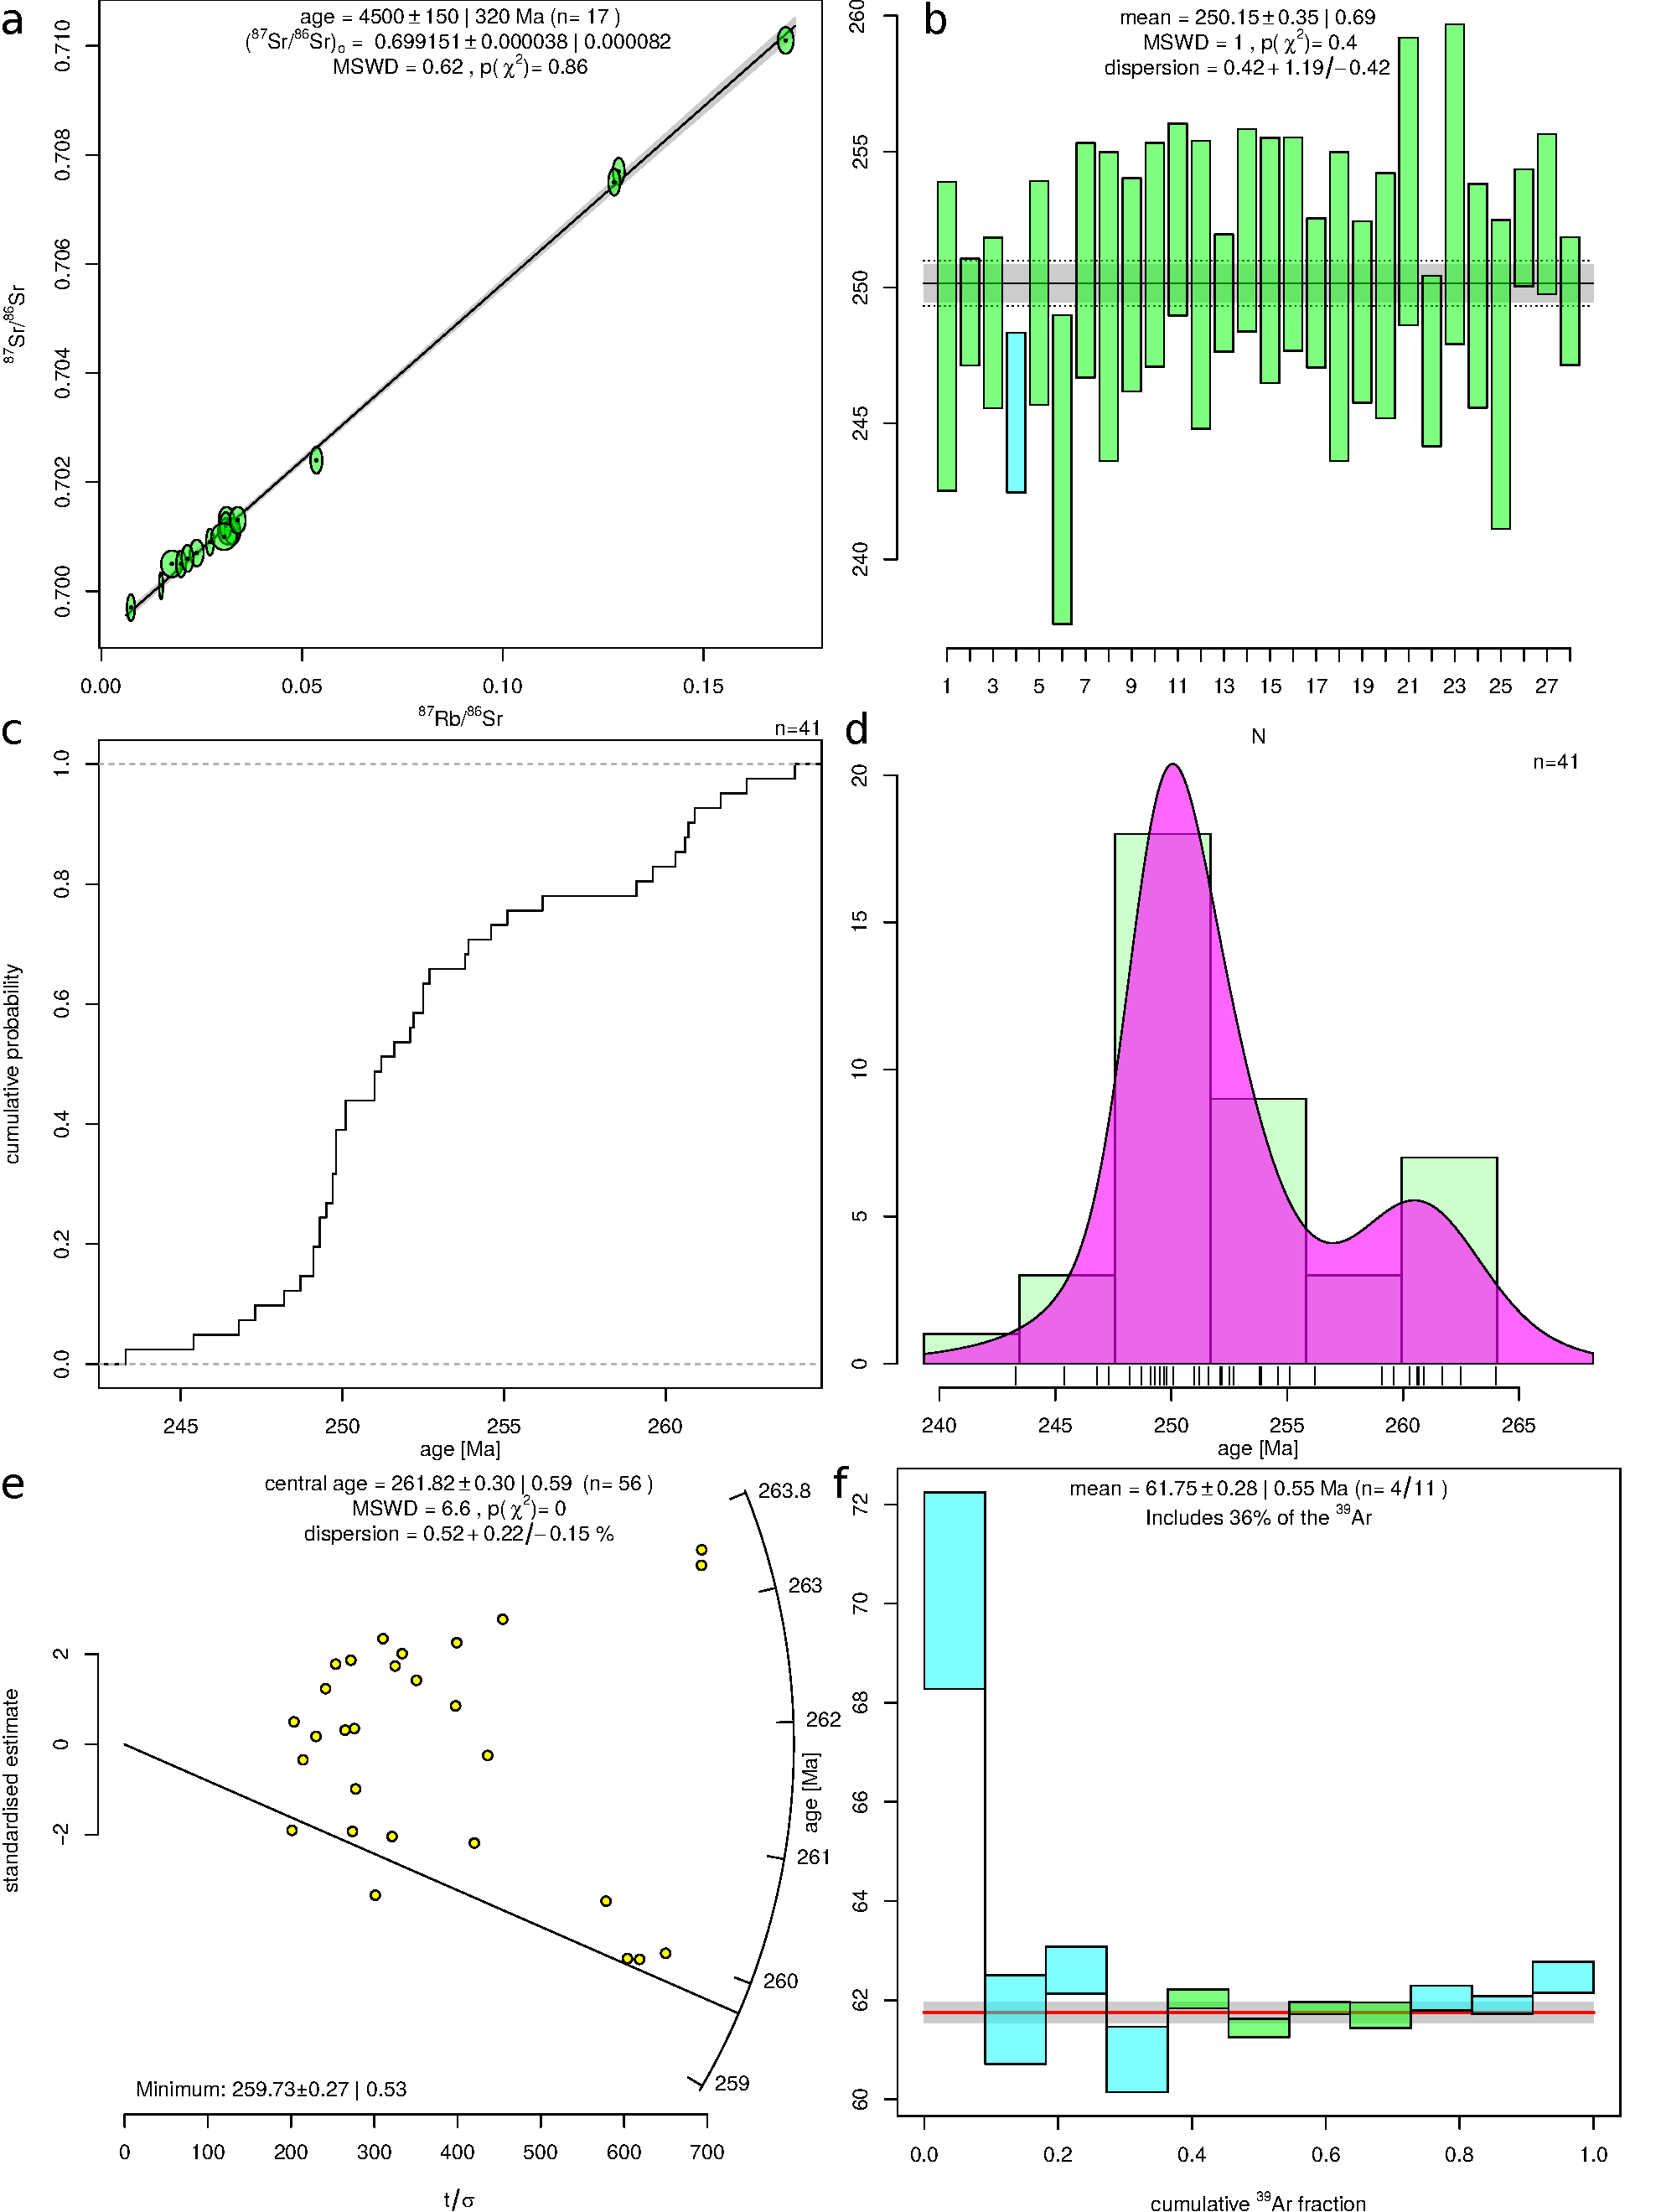
\includegraphics[width=.5\linewidth]{fig1.pdf}
  \caption{
    A--F--M diagram with three decision boundaries between the
    tholeiitic (TH, following the Fenner trend) and calc-alkaline (CA,
    following the Bowen trend) igneous suites. b = basalt, fb =
    ferro-basalt, ab = andesite-basalt, a = andesite, d = dacite and r =
    rhyolite.}
  \label{fig:AFM}
\end{figure}

\section{Logratio processes in igneous petrology}
\label{sec:logratio-processes}

Consider a magma containing $A$ mass units of
Na\textsubscript{2}O+K\textsubscript{2}O, $F$ mass units of
FeO\textsubscript{T}, and $M$ mass units of MgO. Suppose that, as the
magma cools, it loses components $A$, $F$ and $M$ at rates that are
proportional to the amounts of $A$, $F$ and $M$ present in the magma:
\begin{equation}
  \frac{\partial A}{\partial t} = -\lambda_A A \mbox{,~}
  \frac{\partial F}{\partial t} = -\lambda_F F \mbox{,~and~}
  \frac{\partial M}{\partial t} = -\lambda_M M
  \label{eq:decay}
\end{equation}

\noindent where $t$ is time (or, more generally, differentiation
progress) and $\lambda_x$ is a decay constant (for $x \in \{A, F,
M\}$). The same mathematical formulation can be used to describe the
settlement of sediment from a suspension \citep{egozcue2003}, or the
decay of radioactive isotopes \citep{rutherford1902a}.  The solution
to Equation~\ref{eq:decay} is a set of exponential functions:
\begin{equation}
  A = A_\circ \exp(-\lambda_A t) \mbox{,~}
  F = F_\circ \exp(-\lambda_F t) \mbox{,~and~}
  M = M_\circ \exp(-\lambda_M t)
  \label{eq:expdecay}
\end{equation}

\noindent where $A_\circ$, $F_\circ$ and $M_\circ$ are the initial
values of $A$, $F$ and $M$ in the primitive magma
(Figure~\ref{fig:single-stage}a). Different values of $\lambda_A$,
$\lambda_F$ and $\lambda_M$ give rise to different trajectories on the
A--F--M diagram. Combining the three compositional variables $A$, $F$
and $M$ into two logratio variables $\ln(A/F)$ and $\ln(M/F)$ recasts
the exponential functions of Equation~\ref{eq:expdecay} into two
linear functions:
\begin{equation}
\begin{cases}
  \ln(A/F) = & \ln(A/F)_\circ + (\lambda_F-\lambda_A)t\\
  \ln(M/F) = & \ln(M/F)_\circ + (\lambda_F-\lambda_M)t
\end{cases}
\label{eq:simple}
\end{equation}

\noindent which can be combined as follows:
\begin{equation}
  \begin{split}
    \ln(A/F) = & C_1 \ln(M/F) + C_2 \\
    \mbox{where~} C_1 = & \frac{\lambda_F-\lambda_A}{\lambda_F-\lambda_M} \\
    \mbox{and~} C_2 = & \ln(A/F)_\circ - C_1 \ln(M/F)_\circ 
  \end{split}
  \label{eq:linear}
\end{equation}

Thus, the curved trajectories on the AFM diagram become straight lines
in logratio space and vice versa
(Figure~\ref{fig:single-stage}b,c). With an appropriate choice of
initial ratios and decay constants, it is possible to mimic the Fenner
and Bowen trends of the tholeiitic and calc-alkaline magma series,
respectively. This makes geological sense because it is not hard to
imagine how $\lambda_F$ could depend on the oxygen fugacity in the
magma, which controls the valence state of the Fe-ions and, hence, the
minerals that they forms.\medskip

\begin{figure}[!ht]
  \centering
  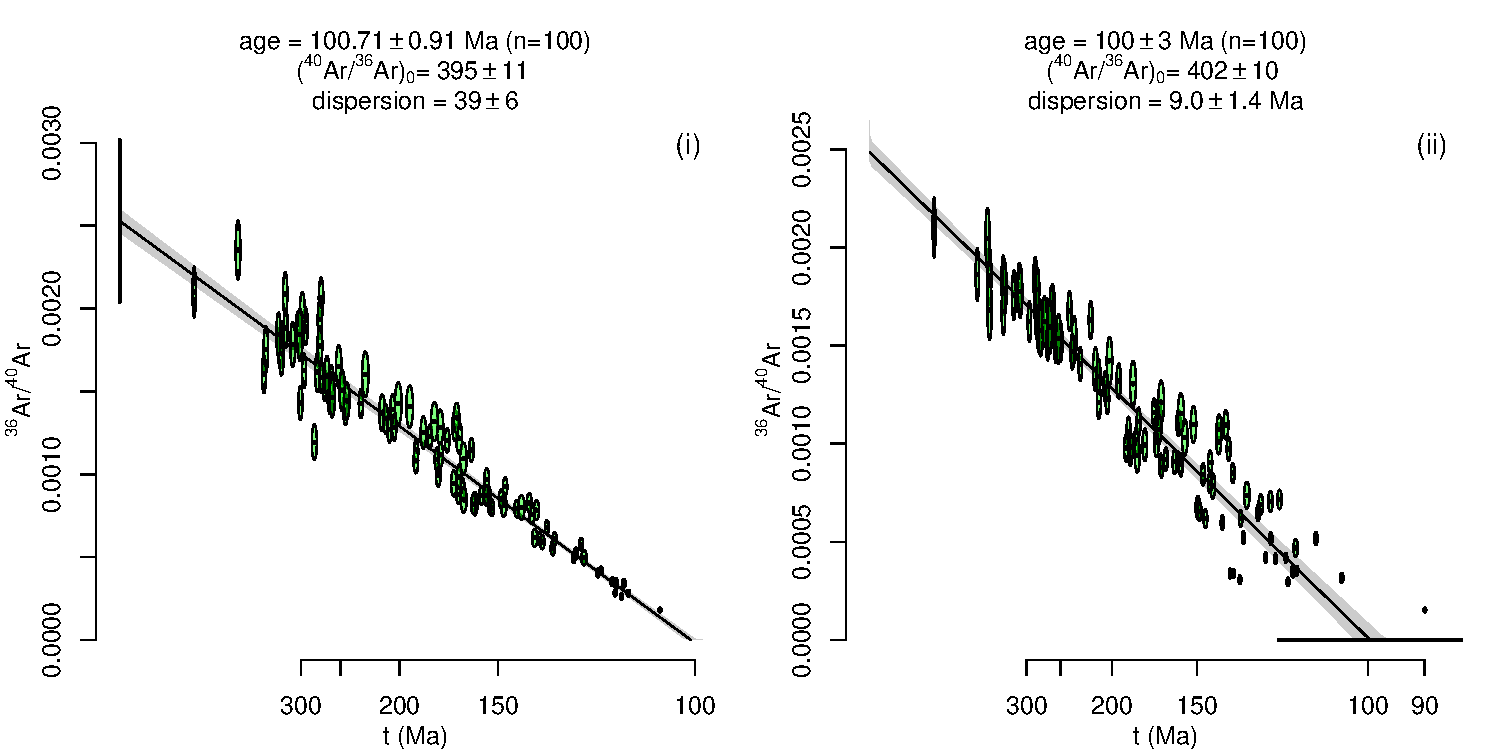
\includegraphics[width=.7\textwidth]{fig2.pdf}
  \caption{ Exponential decay processes of compositional data become
    linear trends in logratio space. a) temporal evolution of a magma
    according to Equation~\ref{eq:expdecay}, with decay constants
    $\lambda_{F}=0.5$ (solid line), $\lambda_{F}=0.7$ (dashed line),
    $\lambda_{M}=0.8$ (dash-dot line) and $\lambda_{A}=0.4$ (dotted
    line); b) removing the time dimension by plotting $\ln(M/F)$
    against $\ln(A/F)$ produces two compositional trends
    (Equation~\ref{eq:linear}) for $\lambda_{F}=0.5$ (solid line) and
    $\lambda_{F}=0.7$ (dashed line); c) mapping these trends to the
    ternary diagram yields two curved trajectories that resemble the
    Fenner and Bowen trends of Figure~\ref{fig:AFM}; d) model fit to
    igneous rock compositions from Iceland (white) and the Cascade
    Mountains (red). Projecting the individual rock compositions onto
    a radial scale gives rise to the Bowen-Fenner ($BF_1$) index,
    which is shown as kernel density estimates (KDEs) for the
    tholeiitic (TH, black) and calc-alkaline (CA, red) samples,
    respectively.}
  \label{fig:single-stage}
\end{figure}

\section{Application to Iceland and the Cascades}

We use the empirical dataset of \citet{rollinson2021} as the basis for
our new model. This dataset includes 456 tholeiitic rocks from Iceland
and 580 calc-alkaline rocks from the Cascade Mountains (see
supplementary material for details). Plotting these compositions on a
diagram of $\ln(M/F)$ vs. $\ln(A/F)$ yields two approximately linear
arrays of data points, as predicted by Equation~\ref{eq:linear}.
Orthogonal regression of these data produces the following trends:
\begin{equation}
  \begin{split}
    \mbox{Fenner:~} \ln(M/F) & = -2.12 - 1.10 \ln(A/F) \\
    \mbox{Bowen:~} \ln(M/F) & = -0.658 - 0.722 \ln(A/F)
  \end{split}
  \label{eq:1stagefit}
\end{equation}

These two lines intersect at $(x_\circ=-3.84, y_\circ=2.12)$, which is
equivalent to a hypothetical common magma source with a normalised
A--F--M composition of ($A_\circ$=0.23\%, $F_\circ$=10.72\%,
$M_\circ$=89.05\%, see Figure~\ref{fig:single-stage}d). This fanning
arrangement of linear trends provides an opportunity to quantify the
degree to which a volcanic rock belongs to the tholeiitic or the
calc-alkaline series. Defining the `single stage Bowen--Fenner
($BF_1$) index' as:
\begin{equation}
  BF_1(A,F,M) =
  9.57 
    \arctan\!\left(
  \frac{
    \ln\!\left({M}/{F}\right)-2.12
  }{
    \ln\!\left({A}/{F}\right)+3.84
  }
  \right) + 6.98
\end{equation}

\noindent projects A--F--M compositions onto a radial scale
(Figure~\ref{fig:single-stage}d), in which the regression line through
the Iceland data is marked by a $BF_1$ index of $-1$, and the
regression line through the Cascades data is marked by a $BF_1$ index
of $+1$. Thus, tholeiitic and calc-alkaline rocks correspond to
negative and positive $BF_1$ values, respectively.\medskip

\begin{figure}[!ht]
  \centering
  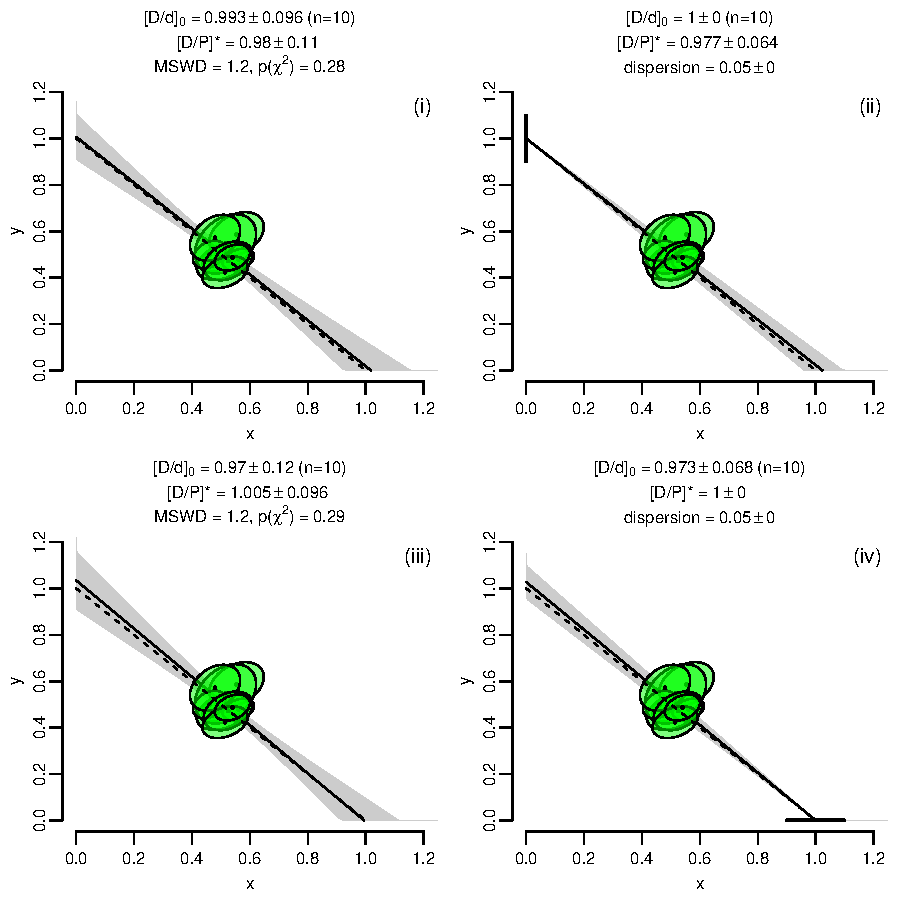
\includegraphics[width=.7\linewidth]{fig3.pdf}
  \caption{ a) the temporal evolution of a two-stage magma evolution
    model (Equation~\ref{eq:temporal}); b) a logratio plot of the
    two-stage model reproduces the characteristic dogleg in the
    tholeiitic magma evolution trend (Equation~\ref{eq:two-stage}); c)
    two-stage model fit to the data of
    Figure~\ref{fig:single-stage}d. Solid blue lines mark the best fit
    of Equation~\ref{eq:FennerBowen}. Dashed blue lines mark the
    decision boundary of Equation~\ref{eq:decision}. $d$ and $D$ are
    the two distances that are needed to compute the $BF_2^F$-index of
    each sample using Equation~\ref{eq:BF2F}. Kernel density estimates
    of the $BF_2^F$-values for the Cascade and Iceland data are shown
    as red and black curves, respectively; d) the two-stage model fit
    transformed back to the ternary diagram.}
  \label{fig:two-stage}
\end{figure}

\section{A two-stage magma evolution model}\label{sec:two-stage}

The fanning arrangement of linear trends shown in
Figure~\ref{fig:single-stage}d successfully discriminates between the
calc-alkaline and tholeiitic magma series. However it is not accurate
in detail, as it fails to capture the prominent dogleg in the
tholeiitic data cloud, which reflects the transition from ferrous to
ferric mineral dominated iron sequestration. Whilst
Equation~\ref{eq:1stagefit} stipulates that the tholeiitic magma
series follows a single linear trend with a different slope than the
calc-alkaline trend, in reality it consists of two linear segments.
The first of these segments has a steeper slope than the calc-alkaline
magma series. It describes the early stages of tholeiitic magma
evolution, during which ferrous Fe is sequestered by minerals such as
olivine and pyroxene. The second segment has the same slope as the
calc-alkaline trend and describes the later stages of tholeiitic magma
evolution, in which ferric Fe is sequestered by magnetite
crystallisation.\medskip

This additional complexity can be captured by modifying the logratio
model of Equations~\ref{eq:decay}--\ref{eq:linear} to form a two-stage
magma evolution history. Let $\lambda_{F2}$ and $\lambda_{F3}$ be the
magmatic decay constant of iron during the first (ferrous) and second
(ferric) stage of magma fractionation, respectively.  And let $f$ mark
the turning point between the first and second stage, where $0<f<1$:
\begin{equation}
\begin{cases}
  \ln(A) = \ln(A)_\circ - \lambda_At &\\
  \ln(M) = \ln(M)_\circ - \lambda_Mt &\\
  \ln(F) = \ln(F)_\circ - \lambda_{F2}t &
  \mbox{~if~} F \leq {f}{F_\circ}\\
  \phantom{\ln(F)}  = \ln(F)_\circ +
  \ln(f)\left[1-\frac{\lambda_{F3}}{\lambda_{F2}}\right] -
  \lambda_{F3}t & \mbox{~if~}F > {f}{F_\circ}
\end{cases}
\label{eq:temporal}
\end{equation}

\noindent then it can be shown that
\begin{equation}
\begin{cases}
  \ln(M/F) = \ln(M/F)_\circ +
  \left[\ln(A/F)-\ln(A/F)_\circ\right]C_3 &
  \mbox{~if~}\ln(A/F) \leq \ln(A/F)_i\\
  \ln(M/F) = \ln(M/F)_\circ + \left[1-C_4\right]C_5 +
  \left[\ln(A/F)-\ln(A/F)_\circ\right]C_4 &
  \mbox{~if~}\ln(A/F) > \ln(A/F)_i
\end{cases}
\label{eq:two-stage}
\end{equation}

\noindent where
\begin{align}
  C_3 = \frac{\lambda_{F2}-\lambda_{M}}{\lambda_{F2}-\lambda_{A}}\mbox{,~}
  C_4 & = \frac{\lambda_{F3}-\lambda_{M}}{\lambda_{F3}-\lambda_{A}}\mbox{,~}
  C_5 = \ln(f)\left[\frac{\lambda_{F3}}{\lambda_{F2}}-1\right]\\ \label{eq:C345}
  \mbox{~and~}
  \ln(A/F)_i & = \ln(A/F)_\circ + \frac{1-C_4}{C_3-C_4}C_5.
\end{align}

Equation~\ref{eq:temporal} describes the temporal evolution of the
two-stage model, which features an inflection point when the
FeO\textsubscript{T} content drops to ${100}\times{f}$\% of its
initial concentration $F_\circ$ (Figure~\ref{fig:two-stage}a). In
Equation~\ref{eq:two-stage}, this inflection point occurs at the
intersection of two linear trends, whose horizontal coordinate is
denoted as $\ln(A/F)_i$ (Figure~\ref{fig:two-stage}b). When
$\lambda_{F2}<\lambda_{F3}$, the logratio pattern reproduces the
distinct dogleg of the tholeiitic magma series
(Figure~\ref{fig:two-stage}b,c).\medskip

The lower FeO\textsubscript{T}-decay constant for the first stage of
the magma evolution model ($\lambda_{F2}$) indicates that the rate at
which iron is withdrawn from the magma is limited by the relatively
low Fe-content of ferrous iron bearing minerals such as olivine and
pyroxene.  Once the magma transitions from a reduced to a more
oxidised state, magnetite starts growing and the (ferric) iron is
extracted from the magma at a higher rate, resulting in the shallower
angle on the logratio diagram.  The calc-alkaline data are dominated
by the second stage, which is parallel to the second stage of the
tholeiitic series. However there is also a faint hint of a dogleg in
the early stages of the calc-alkaline compositions. We can therefore
fit the two-stage model to the calc-alkaline data as well. Joint
optimisation of Equation~\ref{eq:two-stage} using the full
\citet{rollinson2021} dataset yields the following results:
\begin{equation}
  \begin{split}
    \mbox{Fenner:~} \ln(M/F) & = -1.0 - 6.0 [\ln(A/F)+1.45]
    \mbox{~if~} \ln(A/F)\leq{-1.45}\\
    \phantom{\mbox{Fenner:~} \ln(M/F)} & = -1.0 - 0.6 [\ln(A/F)+1.45]
    \mbox{~if~} \ln(A/F)>{-1.45}\\
    \mbox{Bowen:~} \ln(M/F) & = -0.3 - 6.0 [\ln(A/F)+0.80]
    \mbox{~if~} \ln(A/F)\leq{-0.80}\\
    \phantom{\mbox{Bowen:~} \ln(M/F)} & = -0.3 - 0.6 [\ln(A/F)+0.80]
    \mbox{~if~} \ln(A/F)>{-0.80}\\
  \end{split}
  \label{eq:FennerBowen}
\end{equation}

\noindent where, for the sake of parsimony, the two magma evolution
trends are exactly parallel to each other.  The decision boundary
between the tholeiitic and calc-alkaline magma series can then be
defined as the halfway line between these trends:
\begin{equation}
  \begin{split}
    \ln(M/F) & = -0.65 - 6.0 [\ln(A/F)+1.125]
    \mbox{~if~} \ln(A/F)\leq{-1.125}\\
    \phantom{\ln(M/F)} & = -0.65 - 0.6 [\ln(A/F)+1.125]
    \mbox{~if~} \ln(A/F)>{-1.125}\\
  \end{split}
  \label{eq:decision}
\end{equation}

Equations~\ref{eq:FennerBowen} and \ref{eq:decision} are shown on
Figures~\ref{fig:two-stage}c and d as solid and dashed blue lines,
respectively. We can then define the `two-stage Bowen-Fenner index'
($BF_2^F$) as
\begin{equation}
  BF_2^F(A,F,M) = d/D
  \label{eq:BF2F}
\end{equation}

\noindent where $d$ is the signed logratio distance from the sample to
the line defined by Equation~\ref{eq:decision}, and $D$ is half the
distance between the Fenner and Bowen trends of
Equation~\ref{eq:FennerBowen}, measured along the projection line
through the sample composition (Figure~\ref{fig:two-stage}c).

\section{Application to other oxides}

The Ti budget of igneous rocks is controlled by Fe--Ti oxides such as
ilmenite (FeTiO\textsubscript{3}). It is therefore reasonable to
expect a strong link between the temporal evolution of Fe and Ti in
igneous suites.  Indeed, when plotting the \citet{rollinson2021}
dataset on an A--T--M diagram (where T = TiO\textsubscript{2} and A +
T + M = 1), this separates the calc-alkaline and tholeiitic suites
just as well as the A--F--M diagram does. In logratio space, the
dogleg of the tholeiitic rocks is even more prominent than for the
A--F--M data, and is also more noticeable for the calc-alkaline
rocks. Fitting the two-stage magma evolution model to the A--T--M data
yields the following results:
\begin{equation}
  \begin{split}
    \mbox{Fenner:~} \ln(M/T) & = 0.65 + 2.5 \ln(A/T)
    \mbox{~if~} \ln(A/T)\leq{0}\\
    \phantom{\mbox{Tenner:~} \ln(M/T)} & = 0.65 - 0.35 \ln(A/T)
    \mbox{~if~} \ln(A/T)>{0}\\
    \mbox{Bowen:~} \ln(M/T) & = 1.4 + 2.5 [\ln(A/T)-1]
    \mbox{~if~} \ln(A/T)\leq{1}\\
    \phantom{\mbox{Bowen:~} \ln(M/T)} & = 1.4 -0.35 [\ln(A/T)-1]
    \mbox{~if~} \ln(A/T)>{1}\\
  \end{split}
  \label{eq:ATMFB}
\end{equation}

\noindent with the decision boundary again being halfway between these
two lines:
\begin{equation}
  \begin{split}
    \ln(M/T) & = 1.125 + 2.5 [\ln(A/T)-0.5] \mbox{~if~} \ln(A/T)\leq{0.5}\\
    \phantom{\ln(M/T)} & = 1.125 - 0.35 [\ln(A/T)-0.5] \mbox{~if~} \ln(A/T)>{0.5}\\
  \end{split}
  \label{eq:ATMdecision}
\end{equation}

The two linear trends that constitute Equations~\ref{eq:ATMFB} and
\ref{eq:ATMdecision} intersect at an acute angle
(Figure~\ref{fig:ATMfit}a), as opposed to the obtuse angle of
Figures~\ref{fig:two-stage}b and c. This reflects the fact that
$\lambda_T<\lambda_A$ for the first stage and $\lambda_T>\lambda_A$
for the second stage. In contrast, $\lambda_F>\lambda_A$ in both
stages of the A--F--M model
(Figure~\ref{fig:two-stage}a). Equations~\ref{eq:ATMFB} and
\ref{eq:ATMdecision} can be used to define a two-stage Bowen-Fenner
index ($BF_2^T$) in complete analogy with the $BF_2^F$-index of
Equation~\ref{eq:BF2F}. It is also possible to combine the two indices
together to form an average `two-stage Bowen-Fenner index':
\begin{equation}
  BF_2 = (BF_2^F+BF_2^T)/2
\end{equation}

This definition effectively extends the discrimination between the
calc-alkaline and tholeiitic magma series from a three-component
ternary diagram to a four-component compositional
tetrahaedron.\medskip

\begin{figure}[!ht]
  \centering
  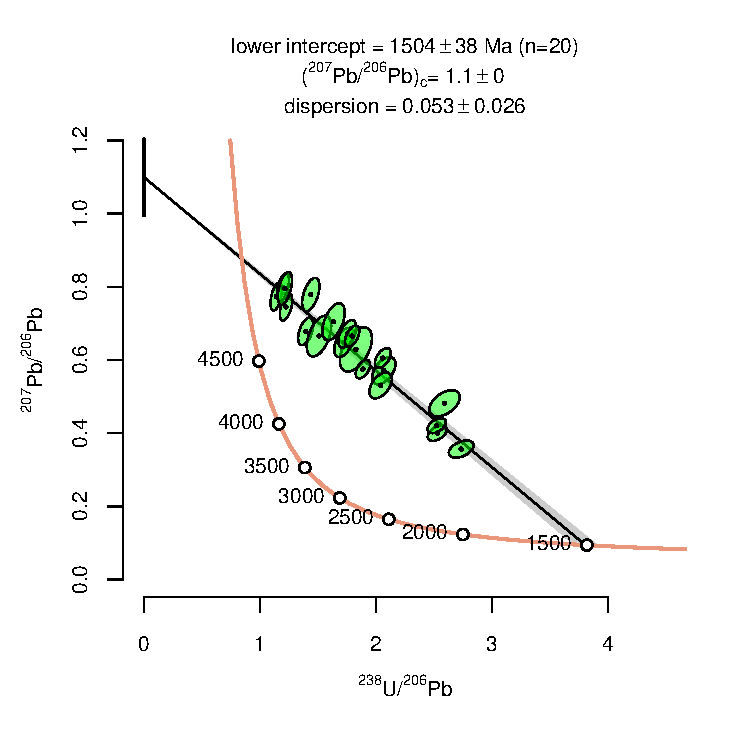
\includegraphics[width=.7\textwidth]{fig4.pdf}
  \caption{ The two-stage magma evolution model of
    Figure~\ref{fig:two-stage} and Equation~\ref{eq:two-stage}, fitted
    to the A--T--M data compilation of \citet{rollinson2021} (where T
    = TiO\textsubscript{2}), shown a) in logratio space and b)
    transformed back to the ternary diagram. Solid blue lines mark the
    best fit of Equation~\ref{eq:ATMFB}. Dashed blue lines mark the
    decision boundary of Equation~\ref{eq:ATMdecision}. The frequency
    distributions of these $BF_2^T$-values are shown as red and black
    kernel density estimates for the Cascade and Iceland data,
    respectively.}
  \label{fig:ATMfit}
\end{figure}

\section{Discussion}

Our method is particularly advantageous because it i) correctly deals
with the statistics associated with closed data sets, ii) is
quantitative, iii) provides better segregation between the two series,
and iv) can be applied to plutonic rocks as well as volcanic
rocks. The logratio models enhance the ability to resolve the
difference between the dacitic and rhyolitic end members of the two
igneous suites, where the Fenner and Bowen trends converge with
increasing alkali content. These trends are well separated in logratio
space, making it easier to distinguish compositions rich in alkali
metals and leading to a more robust boundary in triangular
space.\medskip

As George Box famously said, all models are wrong (but some are
useful) and the simple logratio models presented in this paper are no
exception. The single stage model is clearly wrong because it fails to
capture the distinct dogleg in the tholeiitic magma series.  However
despite this shortcoming, the model effectively discriminates between
the calc-alkaline and tholeiitic magma series. It also serves as a
building block for the more realistic two-stage model, which more
accurately describes the geological mechanism behind the calc-alkaline
and tholeiitic magma series. However, whilst more accurate than the
single stage model, the two-stage model is inevitably also wrong in
its detail. The clean separation into two distinct sets of magmatic
decay constants is an oversimplification. In reality, the transition
between the ferrous and ferric stages is likely to be gradual, not
abrupt.\medskip

Whilst we have formulated our model as a simple function of oxygen
fugacity (via the parameter $f$ in Equations~\ref{eq:temporal} and
\ref{eq:C345}), in reality there are other effects at play. This is
particularly true for the later stages of continental arc magma
evolution where crust-magma interactions can include melts stratified
by density, magma-mixing, crustal assimilation, melt stagnation at the
base of the crust or in the volcano-plutonic plumbing system,
etc. \citep[see discussion in][]{hora2009}. It would be easy to
further improve the fit by adding further parameters, however this
would reduce the numerical stability and geological interpretability
of the model.\medskip

Despite the simplicity of the two-stage model, whose decision
boundaries are completely described by just four numbers, it is highly
successful in discriminating between the calc-alkaline and tholeiitic
magma trends.  Importantly, the same model also describes the
evolution of TiO\textsubscript{2}, leading to a new A--T--M
discrimination diagram.  This success indicates that the exponential
decay functions of Equations~\ref{eq:decay} and \ref{eq:expdecay}
correctly describe the temporal evolution of silicate melts. It
validates the predictive power of genetic (as opposed to purely
empirical) descriptions of magma evolution. The logratio methodology
provides opportunities to investigate other mineral systems, allowing
igneous petrologists to move beyond descriptive geochemistry towards
quantitative models that can be tested in a laboratory setting.\medskip

All the methods presented in this paper have been implemented in
\texttt{R} and can be accessed from
\url{https://github.com/pvermees/GeoplotR/}.

\section*{Acknowledgments}

We would like to thank Julian Pearce and an anonymous reviewer for
their useful comments, which led to the development of the two-stage
model and the addition of the A--T--M diagram to the paper.  This
research was supported by NERC standard grant \#NE/T001518/1.

%\bibliographystyle{/home/pvermees/Dropbox/abbrvplainnat.bst}
%\bibliography{/home/pvermees/Dropbox/biblio.bib}

\begin{thebibliography}{15}
\providecommand{\natexlab}[1]{#1}
\providecommand{\url}[1]{\texttt{#1}}
\expandafter\ifx\csname urlstyle\endcsname\relax
  \providecommand{\doi}[1]{doi: #1}\else
  \providecommand{\doi}{doi: \begingroup \urlstyle{rm}\Url}\fi

\bibitem[Arculus(2003)]{arculus2003}
Arculus, R.~J. (2003)
\newblock Use and abuse of the terms calcalkaline and calcalkalic.
\newblock \emph{Journal of Petrology}, 44, 929--935.

\bibitem[Bowen(1928)]{bowen1928} Bowen, N.~L. (1928) \newblock
  \emph{The Evolution of the Igneous Rocks}.  \newblock Princeton
  University Press.

\bibitem[Egozcue et~al.(2003)Egozcue, Pawlowsky-Glahn, Mateu-Figueras, and
  Barcelo-Vidal]{egozcue2003}
  Egozcue, J., Pawlowsky-Glahn, V., Mateu-Figueras, G., Barcelo-Vidal, C.
  (2003)
\newblock Isometric Logratio Transformations for Compositional Data Analysis.
\newblock \emph{Mathematical Geology}, 35, 279--300.

\bibitem[Fenner(1929)]{fenner1929}
Fenner, C.~N. (1929)
\newblock The crystallization of basalts.
\newblock \emph{American Journal of Science}, 105, 225--253.

\bibitem[Hora et~al.(2009)Hora, Singer, W{\"o}rner, Beard, Jicha, and
  Johnson]{hora2009} Hora, J.~M., Singer, B.~S., W{\"o}rner, G.,
  Beard, B.~L., Jicha, B.~R., Johnson, C.~M. (2009) \newblock {Shallow
    and deep crustal control on differentiation of calc-alkaline and
    tholeiitic magma}.  \newblock \emph{Earth and Planetary Science
    Letters}, 285, 75--86.

\bibitem[Irvine and Baragar(1971)]{irvine1971}
Irvine, T.~N., Baragar, W. (1971)
\newblock A guide to the chemical classification of the common volcanic rocks.
\newblock \emph{Canadian Journal of Earth Sciences}, 8, 523--548.

\bibitem[Kelley and Cottrell(2009)]{kelley2009}
Kelley, K.~A., Cottrell, E. (2009)
\newblock Water and the oxidation state of subduction zone magmas.
\newblock \emph{Science}, 325, 605--607.

\bibitem[Kennedy(1933)]{kennedy1933}
Kennedy, W.~Q. (1933)
\newblock Trends of differentiation in basaltic magmas.
\newblock \emph{American Journal of Science}, 147, 239--256.

\bibitem[Kuno(1968)]{kuno1968}
Kuno, H. (1968) 
\newblock Differentiation of basalt magmas.
\newblock \emph{Basalts: The Poldervaart treatise on rocks of basaltic
  composition}, 623--688.

\bibitem[Osborn(1959)]{osborn1959}
Osborn, E.~F. (1959)
\newblock {Role of oxygen pressure in the crystallization and differentiation
  of basaltic magma}.
\newblock \emph{American Journal of Science}, 257, 609--647.

\bibitem[Pearce and Robinson(2010)]{pearce2010}
Pearce, J.~A., Robinson, P. (2010)
\newblock {The Troodos ophiolitic complex probably formed in a subduction
  initiation, slab edge setting}.
\newblock \emph{Gondwana Research}, 18, 60--81.

\bibitem[Rollinson and Pease(2021)]{rollinson2021}
Rollinson, H., Pease, V. (2021)
\newblock \emph{{Using Geochemical Data to Understand Geological Processes}}.
\newblock Cambridge University Press, 2\textsuperscript{nd} edition.

\bibitem[Rutherford and Soddy(1902)]{rutherford1902a}
Rutherford, E., Soddy, F. (1902)
\newblock The cause and nature of radioactivity -- Part I.
\newblock \emph{The London, Edinburgh, and Dublin Philosophical Magazine and
  Journal of Science}, 21 370--396.

\bibitem[Tilley(1950)]{tilley1950}
Tilley, C. (1950) 
\newblock Some aspects of magmatic evolution.
\newblock \emph{Quarterly Journal of the Geological Society}, 106, 37--61.

\bibitem[Zimmer et~al.(2010)Zimmer, Plank, Hauri, Yogodzinski, Stelling,
  Larsen, Singer, Jicha, Mandeville, and Nye]{zimmer2010}
Zimmer, M.~M., Plank, T., Hauri, E.~H., Yogodzinski, G.~M., Stelling, P.,
  Larsen, J., Singer, B., Jicha, B., Mandeville, C., Nye, C.~J. (2010) 
\newblock {The role of water in generating the calc-alkaline trend: new
  volatile data for Aleutian magmas and a new tholeiitic index}.
\newblock \emph{Journal of Petrology}, 51, 2411--2444.

\end{thebibliography}

\end{document}
